%%%%%%%%%%%%%%%%%%%%%%%%%%%%%%%%%%%%%%%%%
%% Appendix section
% Set-up the section.
\newpage
\appendix
\setcounter{table}{0}
\renewcommand{\thetable}{A\arabic{table}}
\setcounter{figure}{0}
\renewcommand{\thefigure}{A\arabic{figure}}

% Start appendix
\section{Appendix}
\label{appendix}
This project used data which are fully public, and computational tools which are fully open-source.
As such, all code and data involved in this project are available at this project's Github repository, available at \url{https://github.com/shoganhennessy/state-faculty-composition}.
They may be used for replication, or as the basis for further work, as needed.
Any comments or suggestions may be sent to me at \href{mailto:seh325@cornell.edu}{\nolinkurl{seh325@cornell.edu}}, or raised as an issue on the Github project.

A number of statistical packages, for the $R$ language \citep{R2022}, made the empirical analysis for this paper possible.
\begin{itemize}
    \item \textit{Tidyverse} \citep{tidyverse} collected tools for data analysis in the R language.
    \item \textit{LFE} \citep{lfe} implemented linear fixed effect models, with instruments, crucial for the empirical estimation in \autoref{sec:empirics}.
    \item \textit{Stargazer} \citep{stargazer} provided a method to efficiently convert empirical results into presentable output in \LaTeX.
    \item \textit{Lpirfs} \citep{lpirfs2019} implemented estimation of the \cite{jorda2005} local projections methods, with instrumental variables, crucial to the local projections estimates presented in this project.
\end{itemize}


\subsection{First Stage Local Projection Estimates}

\begin{figure}[H]
    \centering
    \singlespacing
    \caption{Local Projection Estimates for First-Stage \autoref{eqn:firststage}.}
    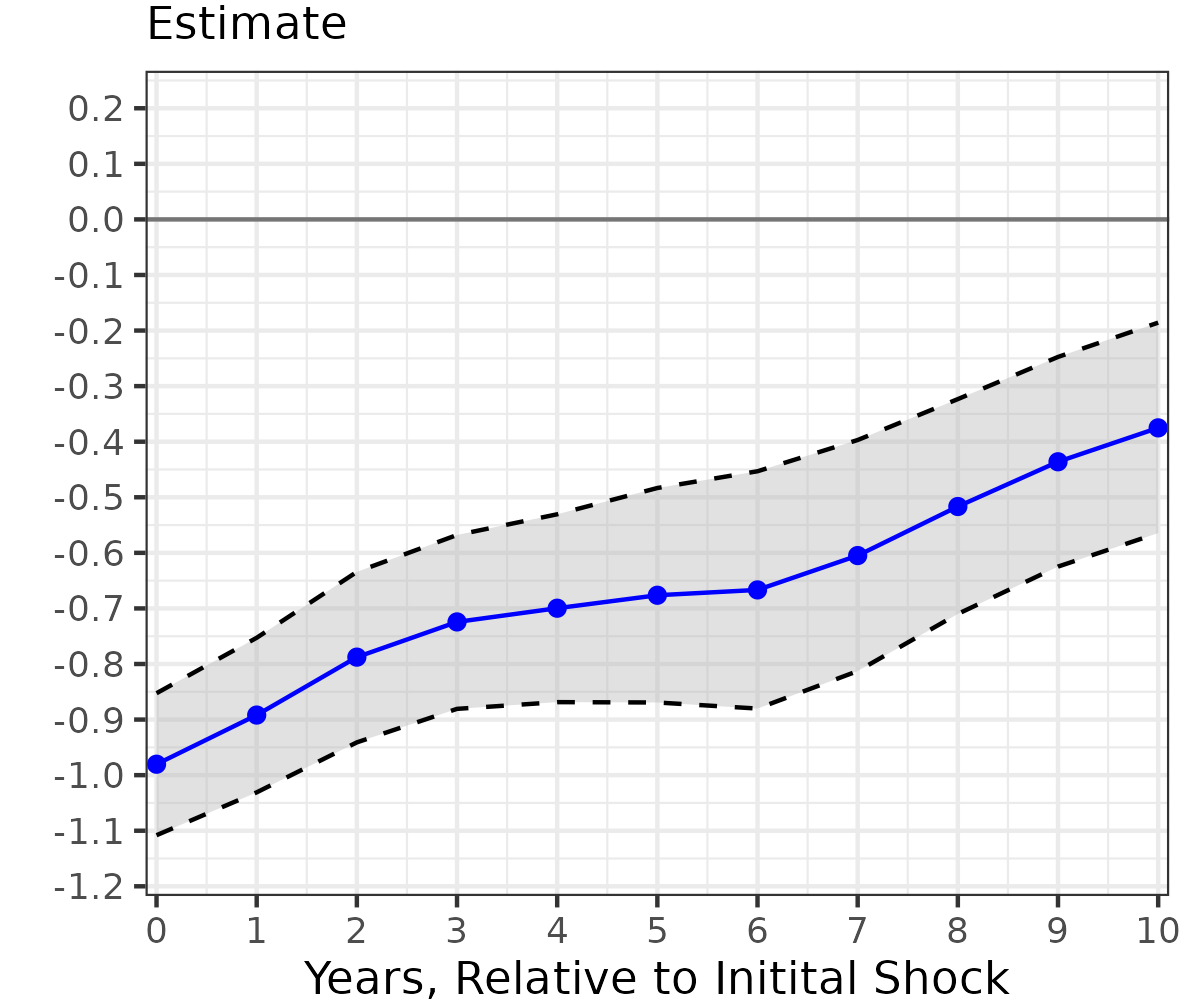
\includegraphics[width=0.6\textwidth]{figures/firststage-lp.png}
    \label{fig:firststage-lp}
\end{figure}


\subsection{First Stage Estimates, Individual Outcomes}
\label{appendix:part1}

\begin{table}[H]
    \singlespacing
    \centering
    \caption{IBHED Summary Statistics, Entire Professor Panel 2010--2021.}
    \makebox[\textwidth][c]{
\begin{tabular}{@{\extracolsep{5pt}}lccc} 
\\[-1.8ex]\hline 
\hline \\[-1.8ex] 
Statistic & \multicolumn{1}{c}{Mean} & \multicolumn{1}{c}{St. Dev.} & \multicolumn{1}{c}{N} \\ 
\hline \\[-1.8ex] 
Lecturer, percent & 38 & 49 & 69,246 \\ 
Assistant professor, percent & 32 & 47 & 69,246 \\ 
Full professor, percent & 13 & 34 & 69,246 \\ 
Administrator professor, percent & 17 & 37 & 69,246 \\ 
Lecturer salary (2021 USD) & 27,714 & 25,715 & 26,324 \\ 
Assistant salary (2021 USD) & 79,661 & 37,138 & 22,328 \\ 
Full salary (2021 USD) & 107,771 & 57,710 & 9,065 \\ 
Administrator salary (2021 USD) & 111,059 & 62,480 & 11,529 \\ 
All salary (2021 USD) & 68,821 & 54,386 & 69,246 \\ 
Lecturer benefits (2021 USD) & 1,925 & 6,966 & 26,324 \\ 
Assistant benefits (2021 USD) & 2,823 & 7,079 & 22,328 \\ 
Full benefits (2021 USD) & 5,861 & 13,440 & 9,065 \\ 
Administrator benefits (2021 USD) & 3,180 & 19,624 & 11,529 \\ 
All benefits (2021 USD) & 2,939 & 11,130 & 69,246 \\ 
\hline \\[-1.8ex] 
\end{tabular} 
}
    \label{tab:illinois-summary-rolling}
    \begin{flushleft}
        \footnotesize
        \textbf{Note}: This table presents the summary statistics for professors with an observed year of first-year at their university.
    \end{flushleft}
\end{table}

\begin{table}[H]
    \singlespacing
    \centering
    \caption{First Stage Estimates, for Total University Revenues at the Individual-Level.}
    \makebox[\textwidth][c]{
\begin{tabular}{@{\extracolsep{5pt}}lcccc} 
\\[-1.8ex]\hline 
\hline \\[-1.8ex] 
 & \multicolumn{4}{c}{Dependent Variable: State Funding} \\ 
\cline{2-5} 
\\[-1.8ex] & (1) & (2) & (3) & (4)\\ 
\hline \\[-1.8ex] 
 Appropriations Shock & $-$0.939 & $-$0.487 & $-$0.920 & $-$0.329 \\ 
  & (0.018) & (0.097) & (0.015) & (0.112) \\ 
  Tuition Revenue & 0.709 & 0.766 &  &  \\ 
  & (0.207) & (0.292) &  &  \\ 
  Constant &  & $-$1.902 &  & 6.477 \\ 
  &  & (3.065) &  & (0.868) \\ 
 \hline \\[-1.8ex] 
Fixed effects? & Yes & No & Yes & No \\ 
F stat. & 2858.843 & 25.057 & 3618.841 & 8.631 \\ 
Observations & 69,246 & 69,246 & 69,246 & 69,246 \\ 
R$^{2}$ & 0.911 & 0.417 & 0.906 & 0.258 \\ 
\hline 
\hline \\[-1.8ex] 
\end{tabular} 
}
    \label{tab:firststage-illinois}
    \begin{flushleft}
        \footnotesize
        \textbf{Note}: Standard errors are clustered at the university-year level.
    \end{flushleft}
\end{table}


\begin{figure}[H]
    \centering
    \singlespacing
    \caption{Local Projection Estimates for First-Stage \autoref{eqn:secondstage1_indiv}.}
    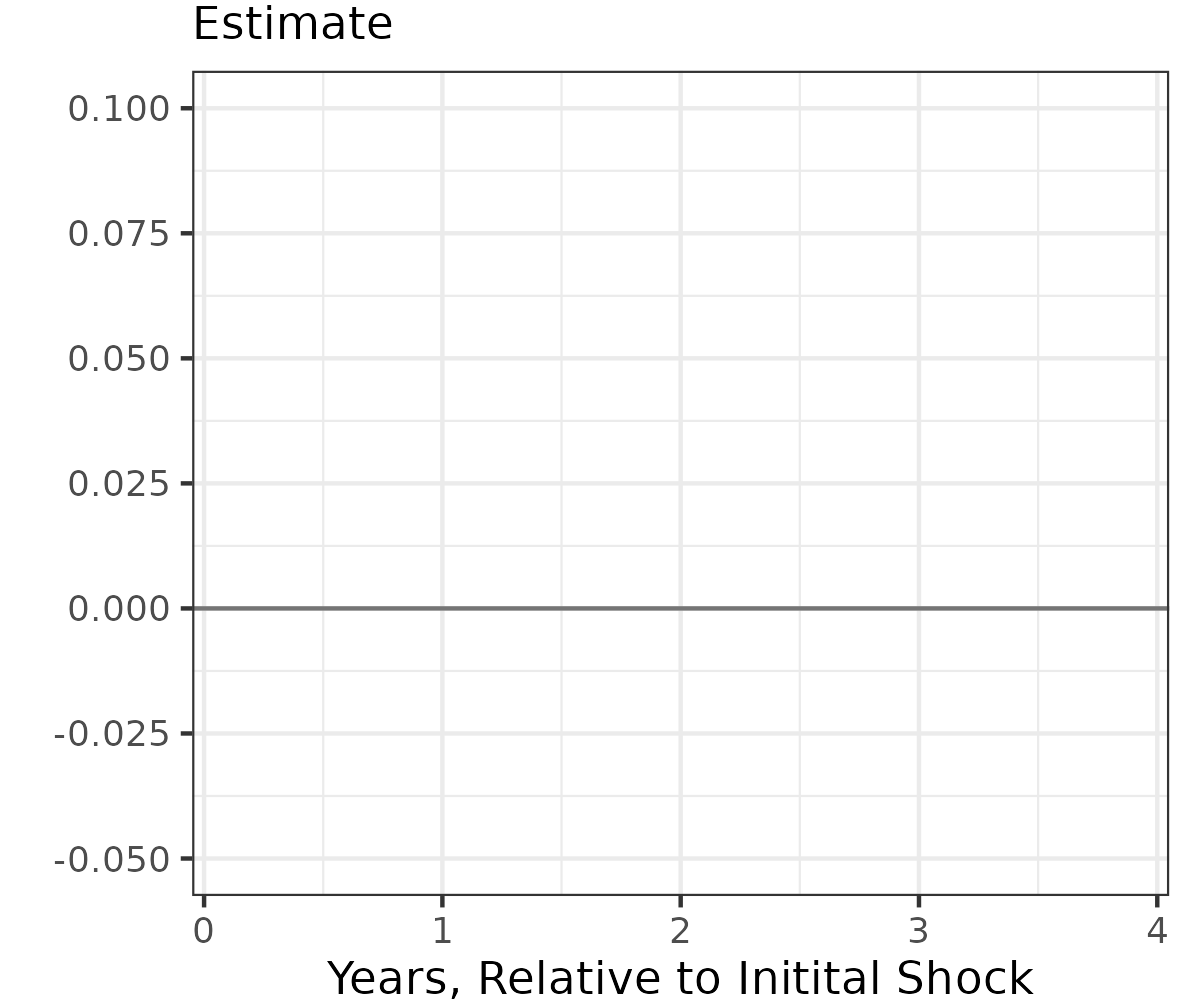
\includegraphics[width=0.6\textwidth]{figures/firststage-illinois-lp-rolling.png}
    \label{fig:firststage-illinois-lp}
\end{figure}


\subsection{Additional Results, University-Level}

\autoref{tab:facultysalaries-shock-reg} presents OLS and IV estimates where the outcome is (log) mean salary for professors employed at the university, separated by position.
Similarly, \autoref{fig:all-salaries-lp} shows the staying-power via projection methods.
The outcome, mean salary is crude.

\begin{table}[H]
    \singlespacing
    \centering
    \caption{OLS and 2SLS Estimates for University Faculty-Tenure Composition.}
    \makebox[\textwidth][c]{
\begin{tabular}{@{\extracolsep{5pt}}lcccccccc} 
\\[-1.8ex]\hline 
\hline \\[-1.8ex] 
 & \multicolumn{8}{c}{Dependent Variable: Employment Count by Tenure Group} \\ 
\cline{2-9} 
\\[-1.8ex] & \multicolumn{2}{c}{Non-tenure} & \multicolumn{2}{c}{Tenure-Track} & \multicolumn{2}{c}{Tenured} & \multicolumn{2}{c}{All} \\ 
 & OLS & 2SLS & OLS & 2SLS & OLS & 2SLS & OLS & 2SLS \\ 
\\[-1.8ex] & (1) & (2) & (3) & (4) & (5) & (6) & (7) & (8)\\ 
\hline \\[-1.8ex] 
 State Funding & 0.003 & 3.332 & 0.045 & 2.367 & 0.051 & 0.886 & 0.043 & 2.925 \\ 
  & (0.017) & (66.670) & (0.049) & (15.854) & (0.028) & (6.337) & (0.029) & (43.349) \\ 
 \hline \\[-1.8ex] 
Observations & 4,633 & 4,633 & 4,851 & 4,851 & 4,878 & 4,878 & 4,906 & 4,906 \\ 
R$^{2}$ & 0.849 & $-$0.419 & 0.782 & $-$1.185 & 0.896 & 0.470 & 0.927 & $-$5.366 \\ 
\hline 
\hline \\[-1.8ex] 
\end{tabular} 
}
    \begin{flushleft}
        \footnotesize
        \textbf{Note}: Standard errors are clustered at the university-year level.
    \end{flushleft}
    \label{tab:tenurecount-shock-reg-fte}
\end{table}

\begin{table}[H]
    \singlespacing
    \centering
    \caption{OLS and 2SLS Estimates for University Faculty Salaries.}
    \makebox[\textwidth][c]{\input{tables/facultysalaries-shock-reg-fte.tex}}
    \begin{flushleft}
        \footnotesize
        \textbf{Note}: Standard errors are clustered at the state-year level.
    \end{flushleft}
    \label{tab:facultysalaries-shock-reg}
\end{table}

\begin{figure}[H]
    \centering
    \singlespacing
    \caption{Local Projection Estimates for Professor Salary, Mean within Each University.}
    \includegraphics[width=0.6\textwidth]{figures/all-salaries-lp.png}
    \label{fig:all-salaries-lp}
\end{figure}

\subsection{Additional Results, Faculty Hiring}
\label{sec:appendix-hiring}

These results were collects by using the open-source network data by \cite{wapman2022quantifying}, summing the count of hires a university made for 2011--2021 across the network structure of the data, and integrating a sum of all revenue related measures from IPEDS data.

\begin{table}[h!]
    \singlespacing
    \centering
    \caption{OLS and 2SLS Estimates for University Faculty Hiring, Total for 2011--2020.}
    \makebox[\textwidth][c]{
\begin{tabular}{@{\extracolsep{5pt}}lcccccc} 
\\[-1.8ex]\hline 
\hline \\[-1.8ex] 
 & \multicolumn{6}{c}{Dependent Variable: Professor Hiring Count} \\ 
\cline{2-7} 
\\[-1.8ex] & \multicolumn{2}{c}{Men} & \multicolumn{2}{c}{Women} & \multicolumn{2}{c}{Total} \\ 
 & OLS & 2SLS & OLS & 2SLS & OLS & 2SLS \\ 
\\[-1.8ex] & (1) & (2) & (3) & (4) & (5) & (6)\\ 
\hline \\[-1.8ex] 
 State Funding & 0.805 & 1.308 & 0.845 & 1.325 & 0.848 & 1.306 \\ 
  & (0.222) & (0.365) & (0.235) & (0.335) & (0.220) & (0.352) \\ 
 \hline \\[-1.8ex] 
Observations & 157 & 157 & 157 & 157 & 157 & 157 \\ 
R$^{2}$ & 0.396 & 0.366 & 0.415 & 0.383 & 0.408 & 0.381 \\ 
\hline 
\hline \\[-1.8ex] 
\end{tabular} 
}
    \begin{flushleft}
        \footnotesize
        \textbf{Note}: Standard errors are clustered at the state level.
    \end{flushleft}
    \label{tab:hiring-shock-reg}
\end{table}

Note that yearly variation is not observed here, so that only the aggregate level, for 180 universities, can be considered.


\subsection{Additional Results, Individual-Professor Level}

\begin{table}[H]
    \singlespacing
    \centering
    \caption{2SLS Estimates for Faculty Salaries at Illinois Universities.}
    \makebox[\textwidth][c]{\input{tables/facultysalaries-shock-illinois.tex}}
    \begin{flushleft}
        \footnotesize
        \textbf{Note}: Standard errors are clustered at the institution-year level.
    \end{flushleft}
    \label{tab:facultysalaries-shock-illinois}
\end{table}

\begin{table}[H]
    \singlespacing
    \centering
    \caption{2SLS Estimates for Faculty Promotion Rate at Illinois Universities, using Rolling Instrument.}
    \makebox[\textwidth][c]{
\begin{tabular}{@{\extracolsep{5pt}}lcccc} 
\\[-1.8ex]\hline 
\hline \\[-1.8ex] 
 & \multicolumn{4}{c}{Dependent Variable: Promotion Rate by Professor Group} \\ 
\cline{2-5} 
 & Lecturer & Assistant & Associate & All \\ 
\\[-1.8ex] & (1) & (2) & (3) & (4)\\ 
\hline \\[-1.8ex] 
 State Funding & 0.015 & 0.036 & 0.029 & 0.016 \\ 
  & (0.007) & (0.019) & (0.065) & (0.008) \\ 
 \hline \\[-1.8ex] 
Observations & 16,420 & 16,972 & 4,340 & 42,132 \\ 
R$^{2}$ & 0.008 & 0.022 & 0.031 & 0.007 \\ 
\hline 
\hline \\[-1.8ex] 
\end{tabular} 
}
    \begin{flushleft}
        \footnotesize
        \textbf{Note}: Standard errors are clustered at the institution and first year of employment level.
    \end{flushleft}
    \label{tab:promotion-shock-illinois-rolling}
\end{table}

\begin{table}[H]
    \singlespacing
    \centering
    \caption{2SLS Estimates for Faculty Promotion Rate at Illinois Universities, using Base-Year Instrument.}
    \makebox[\textwidth][c]{
\begin{tabular}{@{\extracolsep{5pt}}lcccc} 
\\[-1.8ex]\hline 
\hline \\[-1.8ex] 
 & \multicolumn{4}{c}{Dependent Variable: Promotion Rate by Professor Group} \\ 
\cline{2-5} 
 & Lecturer & Assistant & Associate & All \\ 
\\[-1.8ex] & (1) & (2) & (3) & (4)\\ 
\hline \\[-1.8ex] 
 State Funding & 0.013 & 0.035 & 0.027 & 0.015 \\ 
  & (0.007) & (0.017) & (0.039) & (0.009) \\ 
 \hline \\[-1.8ex] 
Observations & 16,420 & 16,972 & 4,340 & 42,132 \\ 
R$^{2}$ & 0.008 & 0.022 & 0.031 & 0.007 \\ 
\hline 
\hline \\[-1.8ex] 
\end{tabular} 
}
    \begin{flushleft}
        \footnotesize
        \textbf{Note}: Standard errors are clustered at the institution and first year of employment level.
    \end{flushleft}
    \label{tab:promotion-shock-illinois}
\end{table}

\begin{figure}[H]
    \centering
    \singlespacing
    \caption{Local Projection Estimates for Promotion Rate at Illinois Universities.}
    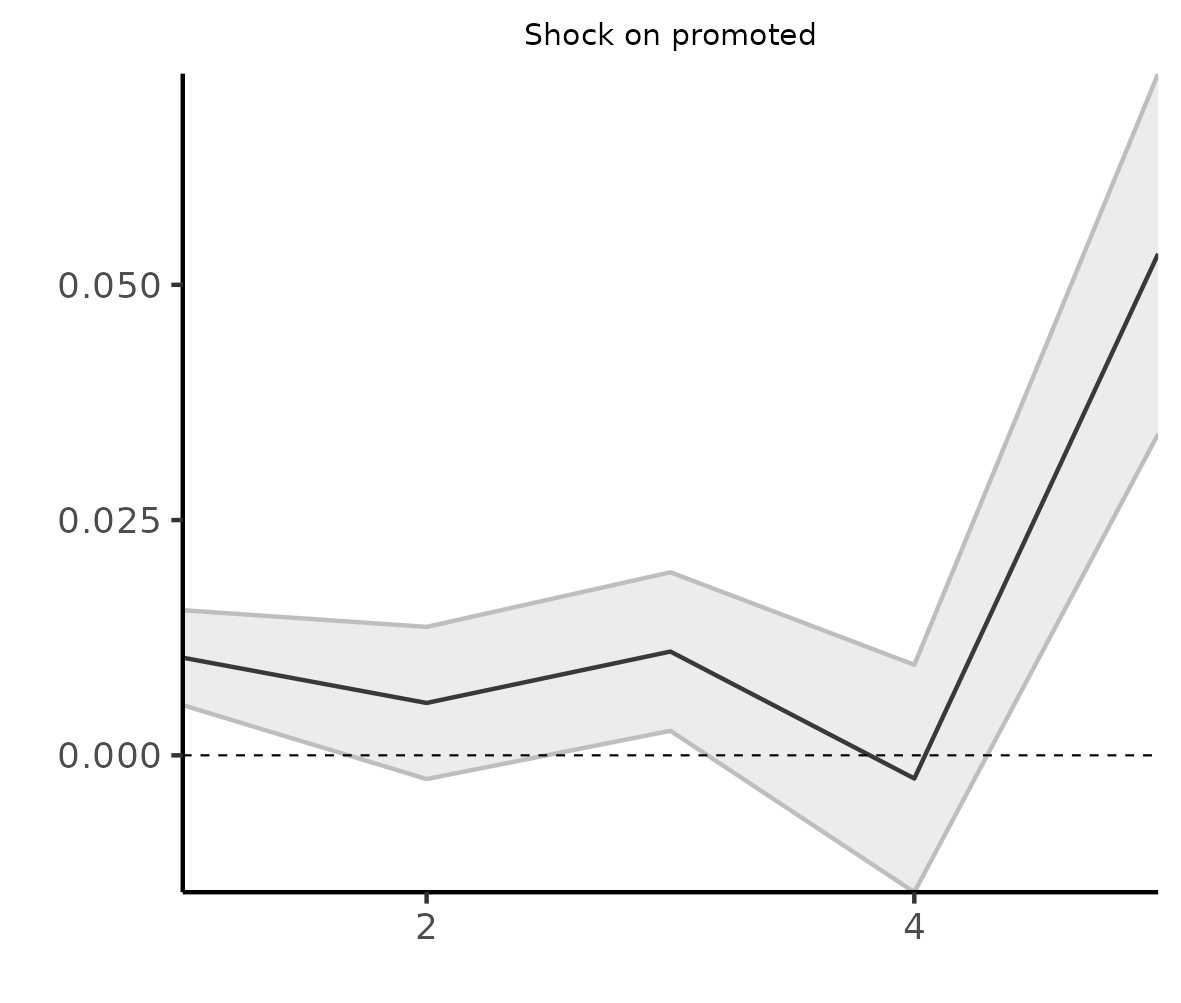
\includegraphics[width=0.6\textwidth]{figures/promoted-illinois-lp-rolling.png}
    \label{fig:promoted-illinois-lp}
\end{figure}

\begin{table}[H]
    \singlespacing
    \centering
    \caption{2SLS Estimates for Faculty Exit Rate at Illinois Universities, using Rolling Instrument.}
    \makebox[\textwidth][c]{
\begin{tabular}{@{\extracolsep{5pt}}lccccc} 
\\[-1.8ex]\hline 
\hline \\[-1.8ex] 
 & \multicolumn{5}{c}{Dependent Variable: Exit rate by Professor Group} \\ 
\cline{2-6} 
 & Lecturer & Assistant & Full & Admin & All \\ 
\\[-1.8ex] & (1) & (2) & (3) & (4) & (5)\\ 
\hline \\[-1.8ex] 
 State Funding & $-$0.003 & 0.003 & $-$0.002 & $-$0.003 & $-$0.004 \\ 
  & (0.024) & (0.007) & (0.009) & (0.020) & (0.016) \\ 
 \hline \\[-1.8ex] 
Observations & 23,841 & 19,904 & 7,244 & 10,241 & 61,230 \\ 
R$^{2}$ & 0.013 & 0.005 & 0.013 & 0.072 & 0.016 \\ 
\hline 
\hline \\[-1.8ex] 
\end{tabular} 
}
    \begin{flushleft}
        \footnotesize
        \textbf{Note}: Standard errors are clustered at the institution and first year of employment level.
    \end{flushleft}
    \label{tab:facultyleaving-shock-illinois-rolling}
\end{table}

\begin{table}[H]
    \singlespacing
    \centering
    \caption{2SLS Estimates for Faculty Exit Rate at Illinois Universities, using Base-Year Instrument.}
    \makebox[\textwidth][c]{
\begin{tabular}{@{\extracolsep{5pt}}lccccc} 
\\[-1.8ex]\hline 
\hline \\[-1.8ex] 
 & \multicolumn{5}{c}{Dependent Variable: Exit rate by Professor Group} \\ 
\cline{2-6} 
 & Lecturer & Assistant & Full & Admin & All \\ 
\\[-1.8ex] & (1) & (2) & (3) & (4) & (5)\\ 
\hline \\[-1.8ex] 
 State Funding & $-$0.021 & $-$0.001 & 0.001 & 0.015 & $-$0.004 \\ 
  & (0.009) & (0.005) & (0.003) & (0.026) & (0.006) \\ 
 \hline \\[-1.8ex] 
Observations & 46,614 & 36,223 & 62,992 & 26,532 & 172,361 \\ 
R$^{2}$ & 0.008 & 0.004 & 0.002 & 0.023 & 0.003 \\ 
\hline 
\hline \\[-1.8ex] 
\end{tabular} 
}
    \begin{flushleft}
        \footnotesize
        \textbf{Note}: Standard errors are clustered at the institution and first year of employment level.
    \end{flushleft}
    \label{tab:facultyleaving-shock-illinois}
\end{table}
